% !TEX TS-program = xelatex
% !TEX encoding = UTF-8 Unicode

% In Class Activity for ME3001- Tristan Hill 
% Spring 2017 - Fall 2017 - Fall 2020 - Fall 2021
% Mechanical Engineering Analysis with MATLAB  and Solidworks
% Module 1 - Introduction and MATLAB Review
% Activity 1 -(In-Class) 

\documentclass[12pt]{article}
\usepackage{/home/thill/Documents/lectures/analysis_lectures/analysis_activities}
%\usepackage{../analysis_activities}

% Title and Misc
\newcommand{\COURNAME}{ME 3001-002}
\newcommand{\CURRTERM}{Fall 2021} %Current Term
\newcommand{\MNUM}{1} %Module Number
\newcommand{\ANUM}{1} %Activity Number
\newcommand{\moduletitle}{Introduction and MATLAB Review}
\newcommand{\activitytitle}{Using the Plot Function} %Module Name
\pagestyle{myheadings}
\markright{{\large ME4140 - ROS Workshop - \CURRTERM}}

\textwidth=7.0in
\topmargin=-0.6in
\leftmargin=0.5in
\textheight=9.25in
\hoffset=-0.5in
\footskip=0.2in

\begin{document}

\thispagestyle{plain}

\begin{center}
   {\bf \Large In-Class Activity\hspc\MNUM\hspc - \activitytitle}\vspace{3mm}\\
   {\bf \large \COURNAME - Mechanical Engineering Analysis - \CURRTERM} \vspace{5mm}\\
\end{center}

\begin{description}

\item[\textbf{\underline{Overview:}}] \hfill \vspace{3mm}\\
You will write a program to generate sample data and graph this data in a correctly formatted scatter plot shown in the figure window.

\item[\textbf{\underline{Learning Objectives:}}] \hfill \vspace{0mm}

\begin{itemize}
	\item You will practice and learn to produce organized graphs to represent a response equation. 
\end{itemize}

\item[\textbf{\underline{Required Materials:}}] \hfill \vspace{0mm}

\begin{itemize}
	\item {\bf Your Computer}: This activity requires a computer with MATLAB or Octave installed.
\end{itemize}

\item[\textbf{\underline{Activity:}}] \hfill \vspace{0mm}

\begin{enumerate}
	

	\item Consider the parabola shown below and write the mathematical function describing the height $y(x)$ and a function of the variable $x$.
	\begin{multicols}{2}

	\[ y(x)=fn(x)= \]


	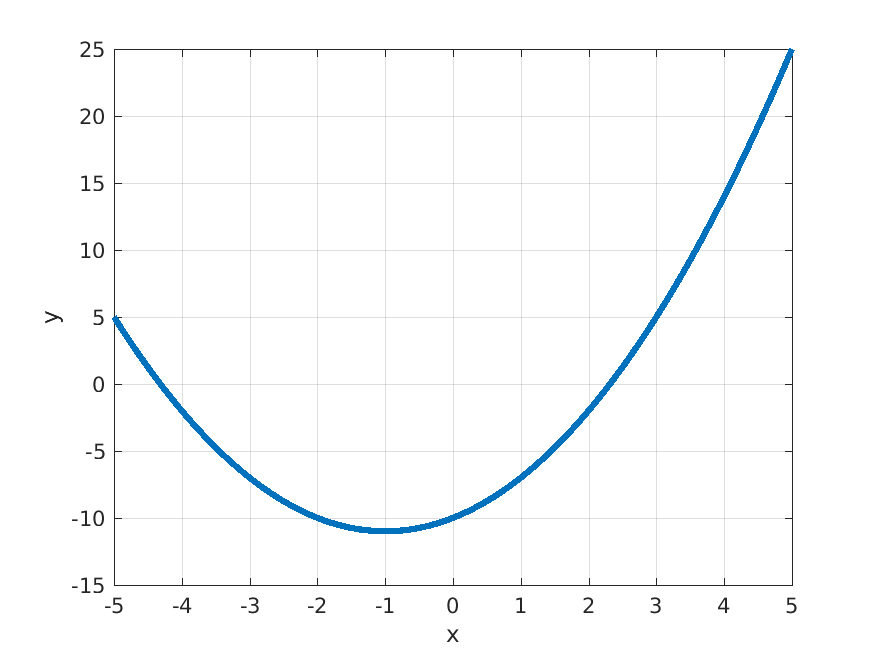
\includegraphics[scale=.5]{activity1_fig1.png}	
	
	\end{multicols}
	
	\item Write a simple MATLAB program named {\bf \BL<USERNAME>\BK\_using\_plot.m} to graph the function in the {\it Figure(1)  window}. Use a range range of x-values ranging from $x=-5$ to $x=5$ and a stepsize that allows the curve to appear smooth. Label all the axes and give the plot a reasonable title.	
	
	\item Estimate or find the values of x that make the function y(x) equal to zero. Show two additional markers on the plot to indicate these points.
	
	\item Save the figure as a PNG file called {\bf \BL<USERNAME>\BK\_using\_plot.png } 
\end{enumerate}

\item[\textbf{\underline{Submit:}}] \hfill \vspace{0mm}

		Submit {\bf \BL<USERNAME>\BK\_using\_plot.m} and {\bf \BL<USERNAME>\BK\_using\_plot.png } to the Activity \ANUM \hspace{1mm} folder before the posted due date.

\end{description}
\end{document}
